\documentclass[UTF8]{ctexart}
\usepackage[a4paper,left=3cm,right=3cm,top=2cm]{geometry}
\usepackage{amsmath}
\usepackage{enumitem}
\usepackage{float}
\usepackage{threeparttable}
\usepackage{caption}
\usepackage{multirow}
\usepackage{graphicx}
\usepackage{listings}
\usepackage{xcolor}
\usepackage{amssymb}
\renewcommand{\figurename}{Figure}
\definecolor{dkgreen}{rgb}{0,0.6,0}
\definecolor{gray}{rgb}{0.5,0.5,0.5}
\definecolor{mauve}{rgb}{0.58,0,0.82}
\lstset{frame=tb,
  language=C++,
  aboveskip=3mm,
  belowskip=3mm,
  showstringspaces=false,
  columns=flexible,
  basicstyle={\small\ttfamily},
  numbers=left,%设置行号位置none不显示行号
  %numberstyle=\tiny\courier, %设置行号大小
  numberstyle=\tiny\color{gray},
  keywordstyle=\color{blue},
  commentstyle=\color{dkgreen},
  stringstyle=\color{mauve},
  breaklines=true,
  breakatwhitespace=true,
  escapeinside=`,%逃逸字符(1左面的键),用于显示中文例如在代码中`中文...`
  tabsize=4,
  extendedchars=false %解决代码跨页时,章节标题,页眉等汉字不显示的问题
}

\setlength\lineskiplimit{5.25bp}
\setlength\lineskip{5.25bp}

\title{Lab08 Report}
\author{崔士强 PB22151743}
\date{January 14, 2024}

\bibliographystyle{plain}

\begin{document}

\maketitle
\section{Purpose}
The purpose of the program is to implement Lab01 through Lab04 using C++.

Anticipated outcomes: Consistent with outcomes in corresponding lab.

\section{Principles}
Approaches to solve the problems have been discussed in previous lab reports. So here we only focus on the  
high-level language implementation of those approches.

\subsection{Lab01 Counting Zero}
Initialize an integer \lstinline{singleBit} with 1. Then obtain 
a number with only the $(n+1)^{th}$ bit being $1$ in binary representation. Perform bit-wise AND with the
given number to get the information on the corresponding bit.

Relevant code:
\begin{lstlisting}[caption = {Lab01}]
int16_t lab1(int16_t n) {
    // initialize
    int16_t singleBit = 1;
    int count = 0;

    // calculation
    if((n & 1) == 0)      n = -n;     // odd number
    for(int i = 0; i < 16; i++){
        count = count + !(n & singleBit);
        singleBit = singleBit + singleBit;
    }

    // return value
    return count + STUDENT_ID_LAST_DIGIT;
}
\end{lstlisting}

\subsection{Lab02 The PingPong Sequence}
Use an indicator \lstinline{operator_d_n} to indicate the current operator(i.e. $d_n$). Check
for divisibility by $8$ and the last digit by repeatedly substracting 8 and 10 respectively, as in Lab02.

Relevant code:
\begin{lstlisting}[caption = {Lab02}]
int16_t lab2(int16_t n) {
    // initialize
    int16_t result = 3;
    int operator_d_n = 1;    // 1 for +, -1 for -

    // calculation
    for( ; n>1; n--){
        if(operator_d_n == 1)    result = result + result + 2;
        else    result = result + result - 2;
        result = result & 0x0FFF;
        if(Check4LastDigit(result)||Check4Divisibility(result))   operator_d_n = -operator_d_n;
    }

    // return value
    return result;
}

bool Check4LastDigit(int16_t result){
    while(result>0)   result = result - 10;
    return result == -2;
}

bool Check4Divisibility(int16_t result){
    while(result>0)   result = result - 8; 
    return result == 0;
}
\end{lstlisting}

\subsection{Lab03 String Compare}
Use a loop to check the characters at the same position in two given strings.

Relevant code:
\begin{lstlisting}[caption = {Lab03}]
int16_t lab3(char s1[], char s2[]) {
    // initialize
    int i = 0;

    // calculation
    while(s1[i] == s2[i]){
        if(s1[i++] == '\0')   return 0;
    }

    // return value
    return s1[i]-s2[i];
}
\end{lstlisting}

\subsection{Lab04 Baguenaudier}
Implement two functions \lstinline{void Put()} and \lstinline{void Remove()}. These two 
functions recursively call themselves according to the rule.



\section{Procedure}
\subsection{Bugs encountered}
In the implementation of Lab02, the program ran into an infinite loop. The problem was that 
condition for a \lstinline{while} loop was not set correctly:
\begin{lstlisting}
bool Check4LastDigit(int16_t result){
    while(result)   result = result - 10;
    return result == -2;
}
\end{lstlisting}
In this case the loop would continue after \lstinline{result} reaches nagative.

Correction: Change \lstinline{result} to \lstinline{result>0}.

\section{Results}
Testcases are as follows:
\begin{lstlisting}
  5
  15
  6280
  1
  15
  24
  zfz gfg
  bfb bfb
  DsTAs DsTA
  3
  5
  7
\end{lstlisting}
\clearpage
Results: 
\begin{figure}[H]
  \centering
  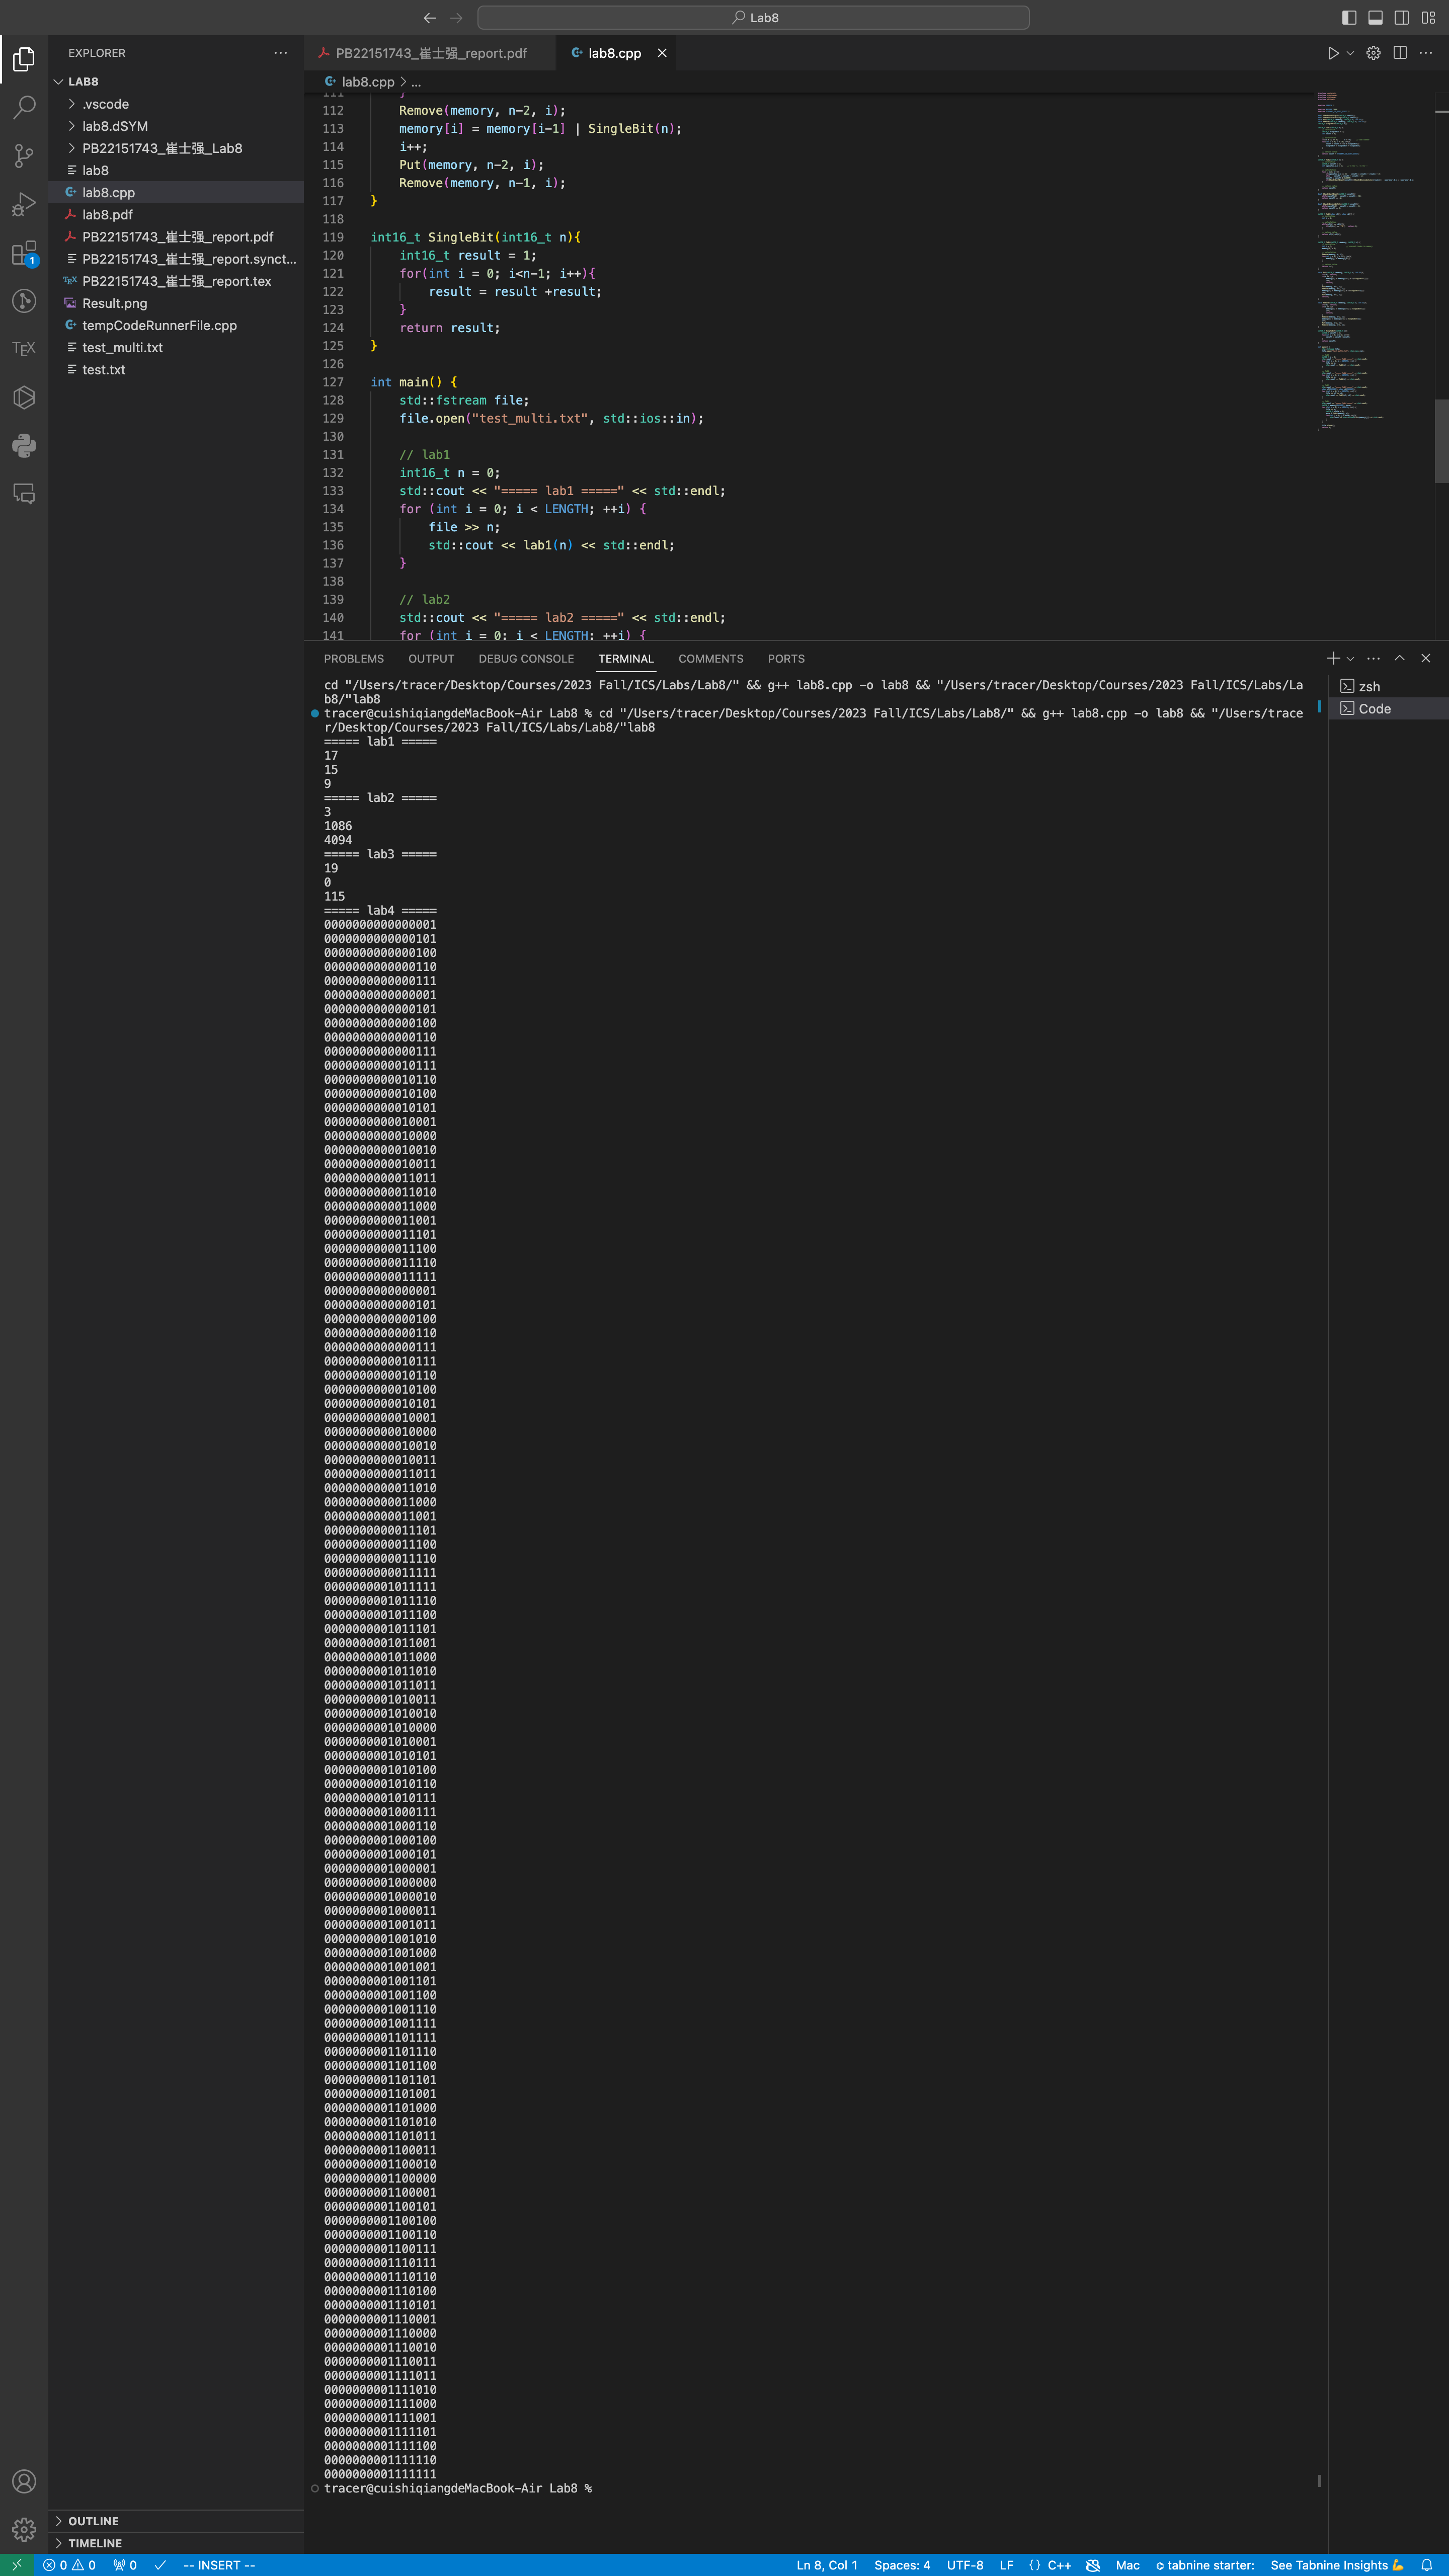
\includegraphics[scale=0.23]{Result.png}
  \caption{Result}
\end{figure}

\bibliography{math}

\end{document}
\iffalse
\begin{figure}[H]
    \centering
    \includegraphics[scale=0.5]{name.png}
    \caption{name}
\end{figure}
\fi
